As we have seen before, MALIS performs really well, but can still be
improved.\\
It was most notably improved in~\cite{funke_large_2019} where they were able to
improve the affinity prediction using more recent architectures, by improving
the training and taking full advantage of the MST and by applying a
post-processing on the affinity graph instead of a simple thresholding.

\begin{figure}[!htbp]
	\centering
	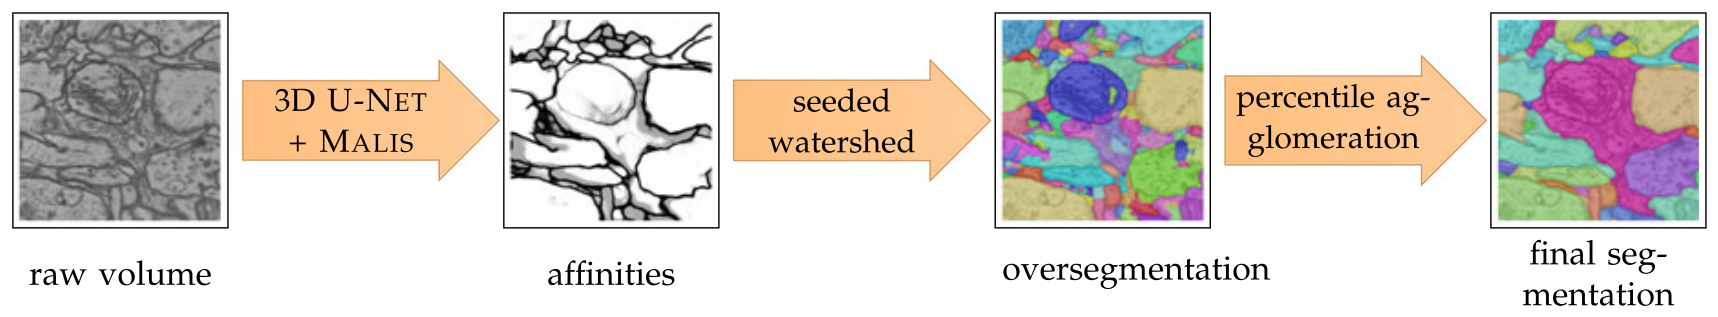
\includegraphics[width=0.8\linewidth]{./images/mala_process.png}
	\caption{Improves MALIS as described in~\cite{funke_large_2019}}%
	\label{fig:mala_process}
\end{figure}

As we can see in figure~\ref{fig:mala_process} the CNN was replaced by a U-Net,
which we will describe afterwards. Then the segmentation is obtained using a
seeded-watershed, which is then improved using a percentile agglomeration of
small objects.

\subsection{Using a more potent architecture}
Indeed, one of the limits of the previous method was the use of a relatively
simple neural network to predict the affinity. This is mostly due to the fact
that neural networks have greatly improved since the original
paper~\cite{turaga_maximin_2009} in 2009.\\

\begin{figure}[!htbp]
	\centering
	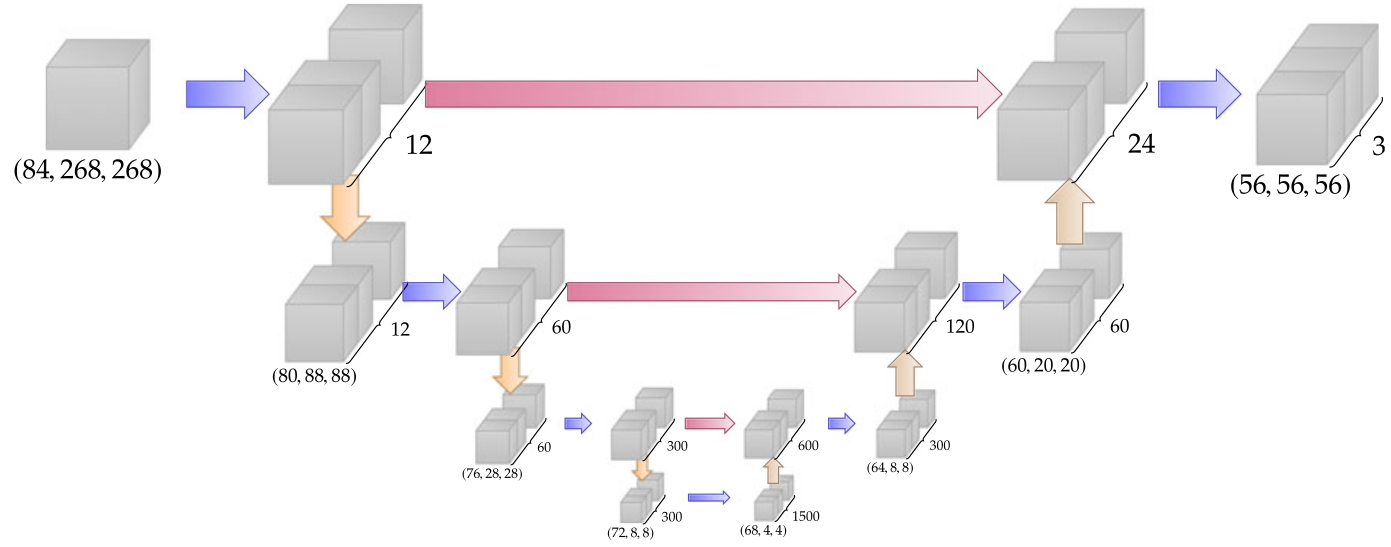
\includegraphics[width=0.8\linewidth]{./images/mala_architecture.png}
	\caption{U-Net architecture used on the CREMI dataset from~\cite{funke_large_2019}}%
	\label{fig:mala_unet}
\end{figure}


U-nets especially have been widely used for image segmentation and are thus a
natural choice in our case. The architecture used in~\cite{funke_large_2019}
is shown in figure~\ref{fig:mala_unet}. As we can see, the training will
obviously be much longer than previously, but the results should be
significantly better.\\
A question that can arise is why not simply use just a U-Net without the MALIS
loss, and as we will see later, the MALIS loss gives us better results on
differents measures of segmentation quality.


\subsection{Constrained MALIS loss}

Previously, we only computed the maximin edge for a pair of pixels (or a finite
amount of pairs), which means that some information from the MST was not
used.\\
However, we would like to compute the maximin edge for all pairs of pixels in
the image. This was not done in the previous paper for time efficiency
reasons.\\
However they describe a way to compute the loss with in quasilinear time instead
of in polynomial time.\\

The main idea is that all maximin edges are in the MST, and there are $n-1$
edges if we have $n$ pixels in our image. We could then simply compute the loss
over all those edges but this would mean that they are all as important as the
others. However since we have $n^2$ pairs of points and $n-1$ edges in our MST,
they will be the maximin edge for a different number of pixel-pairs. So we must
find a way to see how often an edge from the MST is a maximin edge.\\

When we add an edge using Kruskal's algorithm, we can look at the "size" of the
trees it merges and deduce the number of pairs for which the current edge is
the maximin edge.\\

From this, we can define the positive weight of an edge $e$ as the number of pairs
from the same object/segment merged by adding $e$ to the MST. More formally we
have :
\begin{equation*}
	w_p(e)=\lvert \{(u,v)\in F^2 \;|\;\delta(u,v)=1, e=mm(u,v) \}   \rvert
\end{equation*}

Similarly we can define the negative weight of an edge as :
\begin{equation*}
	w_n(e)=\lvert \{(u,v)\in F^2 \;|\;\delta(u,v)=0, e=mm(u,v) \}   \rvert
\end{equation*}

These formulations allow us to rewrite our loss function as :

\begin{equation*}
	L(I,\theta,S) = \sum_{e\in MST(G)} w_p(e)l(1,A_e(I,\theta)) + w_nl(0,A_e(I,\theta))
\end{equation*}
With $A_e$ the affinity of an edge $e$.\\

\textbf{\textcolor{red}{Explain how to compute wn and wp}}
\\

With this loss function being able to be computed in quasilinear time, this
will allow us to use the whole patch for the loss computation instead of a few
pairs of pixels, which should improve the results. This loss function is the
same as before, it still is related to the Rand Index, but it should now
approximate it much better.\\

\subsection{Two pass computation of the loss}


\subsection{Seeded watershed as post processing}

Remember that before, we computed the segmentation by thresholding our affinity
graph. However this doesn't give optimal results, as for example locally
another threshold would perform better.\\
An issue that was also encountered was small objects that were inside bigger
ones. These objects lead to an oversegmentation and we would like a way to
automatically remove those inaccuracies, or at least part of them.

\begin{figure}[!htbp]
	\centering
	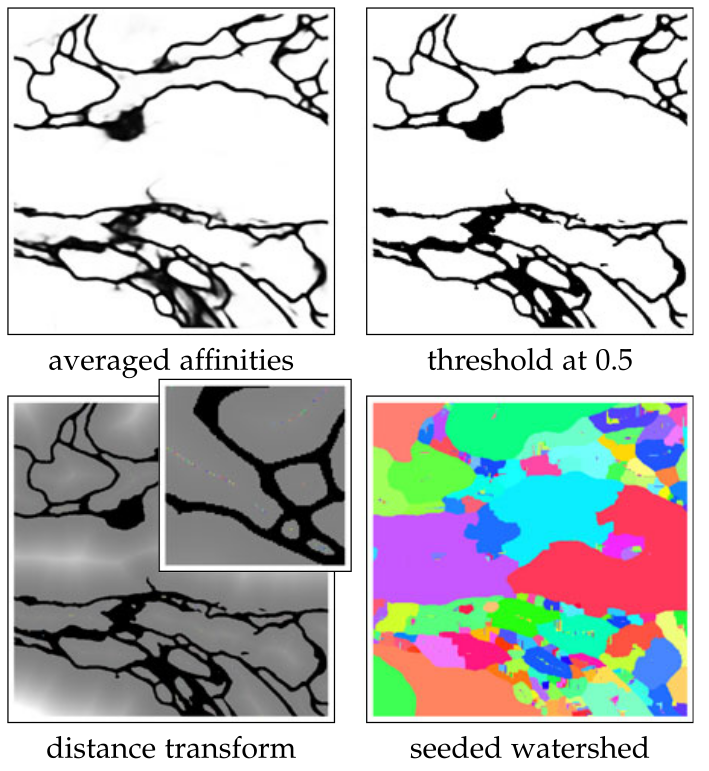
\includegraphics[width=0.5\linewidth]{./images/mala_post_proc.png}
	\caption{Seeded watershed on an affinity graph, as described in~\cite{funke_large_2019}}%
	\label{fig:seeded_ws}
\end{figure}

This is where the framework described in~\cite{funke_large_2019} comes in play.
As we can see in figure~\ref{fig:seeded_ws}, the first step of the process is
to average the affinities, as we did before. Afterwards the averaged affinities
are thresholded at 0.5 (here this threshold is not a parameter). Then a
distance transform (or a distance map) is computed from the objects to the
borders. In this distance transform, the furthest points from the borders will
have the higher values. Then, all the local maxima are taken as seeds for a
seeded watershed, which gives us a first segmentation.\\

This is still an oversegmentation, but a fragment agglomeration algorithm is
then used to fuse regions together. multiple criteria can be used to
determine which regions to merge together and they are described
in~\cite{funke_large_2019}.\\
When all of those steps are done, we obtain the final segmentation.\\

\textbf{\textcolor{red}{Describe agglomeration}}
\\

As we can see the process is greatly improved from the first version of MALIS,
with the loss function, the neural network architecture and the post processign
used being much more powerful than their previous counterparts.
